\chapter{Equilibrium}

\section{Rod and spring}
\begin{problem}
  In \cref{fig:rodspring}, a uniform rod of mass \qty{8.0}{\kg} and
  length \qty{0.50}{\metre}
  is pivoted about point \(P\). It is held in position by a spring of
  original length \qty{0.20}{\metre},
  spring constant \qty{5.0e2}{\newton\per\metre}, and negligible mass.
  Determine the length \(x\).
\end{problem}
\begin{wrapfigure}{i}{0.5\textwidth}
  \centering
  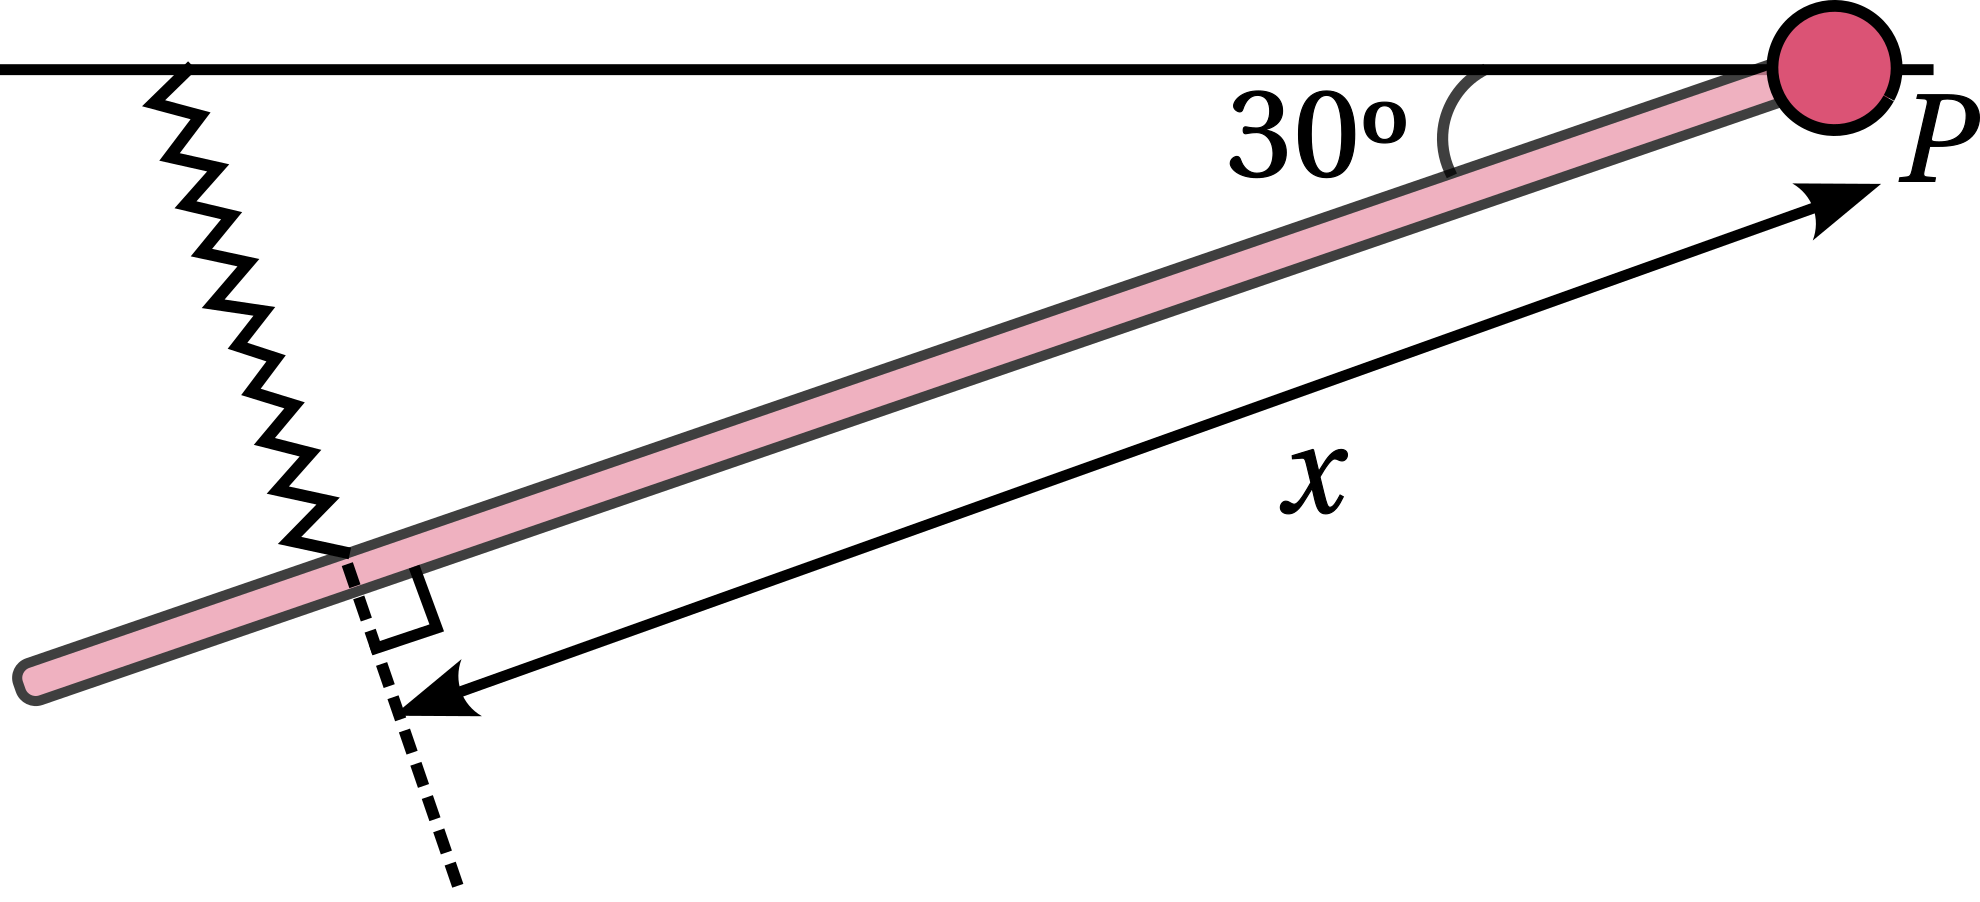
\includegraphics[width=0.48\textwidth]{assets/rodspring.png}
  \caption{Rod and spring}
  \label{fig:rodspring}
\end{wrapfigure}
We define our variables. Let
\begin{itemize}
  \item \(e\) be the extension of the spring, \(l_s\) be its original
    length, and \({l_s}'\) be its stretched length;
  \item \(k_s\) be the spring constant;
  \item \(m\) be the mass of the rod, and \(l_r\) be its length; and
  \item \(\theta\) be the angle the rod makes with the wall.
\end{itemize}

The stretched spring, the rod (up to a distance \(x\) away from the
pivot) and the wall
form a right-angled triangle. The stretched length \({l_s}' = x \tan \theta\).
Therefore, the extension of the spring \(e = {l_s}'-l_s = x\tan\theta - l_s\).

The elastic force generated by the spring \(F_s\) is determined to be
\begin{equation}
  \mv{F}_s = k_se = k_s\ab(x\tan\theta-l_s)
  \label{eq:elastic}
\end{equation}

Also acting on the body of the rod, the weight of the rod \(\mv{W} = mg\). Since
the rod's weight does not act perpendicularly to the rod in this instance, we
can resolve its weight into its vertical component. Furthermore, since the rod
is \term{uniform}, its weight acts in the geometrical centre of its
body, a distance \(\lf{l_r}{2}\)
away from the pivot \(P\).

Since the rod is held in position, it must be in \term{rotational
equilibrium}---the
sum of moments about the pivot \(P\) must equal \(0\). The following
condition in \cref{eq:roteqrule} must hold true.
\begin{equation}
  \sum\tau = 0
  \label{eq:roteqrule}
\end{equation}

Taking the moments generated by the spring's elastic force in
\cref{eq:elastic} and
the rod's weight, we obtain from \cref{eq:roteqrule} that
\begin{align*}
  \sum\tau &= \tau_{\mv{F}_s} + \tau_{\mv{W}_y} \\
  &= \mv{F}_s\cdot x - \mv{W}\cos\theta\cdot\f{l_r}{2} \\
  &= k_sx\ab(x\tan\theta - l_s) - \f{mgl_r\cos\theta}{2} \\
  &= 0 \\
  \ab(k_s\tan\theta)x^2 - k_sl_sx -\f{mgl_r\cos\theta}{2} &= 0\\
  x&= \f{k_sl_s + \sqrt{\ab(k_sl_s)^2 + 2k_smgl_r\sin\theta}}{2k_s\tan\theta} \\
  &= \hil{\qty{0.471}{\metre}}
\end{align*}

\section{Baby stroller}
\begin{problem}
  The diagram shows the side view of a baby stroller. The combined
  mass of stroller and the boy is \(m = \qty{22.0}{\kilo\gram}\). The centre
  of gravity of the boy and stroller lies \qty{0.40}{\metre} in front
  of the hind wheels
  and \qty{0.35}{\metre} above the ground.

  Determine the forces experienced by the front wheels \(F_1\) and
  the hind wheels
  \(F_2\) respectively from the ground.
\end{problem}

For the stroller to remain in equilibrium, \term{translational equilibrium}
and \term{rotational equilibrium}
must be attained. In static equilibrium, the \it{vertical} forces
must sum to \(0\):
\begin{equation}
  F_1 + F_2 = mg
  \label{eq:stateq}
\end{equation}

Moments about a pivot outside of the body of the mass can be found by
extending the line of action
of the force. In {rotational equilibrium}, the sum of moments about
the pivot---here we choose
the centre of gravity--must equal \(0\).
\begin{align}
  F_1\ab[1.0-\ab(0.40-0.30)] - F_2\ab(0.40-0.30)&=0 \\
  0.9F_1 - 0.1F_2&=0
  \label{eq:roteq}
\end{align}

Solving \cref{eq:stateq} and \cref{eq:roteq} simultaneously, we obtain
\begin{align*}
  F_1 &= 0.1mg = \hil{\qty{21.6}{\newton}} \\
  F_2 &= 0.9mg = \hil{\qty{194}{\newton}}
\end{align*}

\begin{problem}
  As the stroller is not easy to manoeuvre, it is common to see parents
  hanging their groceries at the handle to free their hands.
  Determine the maximum load, \(M\), that can be placed at the handle
  before the stroller topples over.
\end{problem}

The total mass of the stroller and all its components is now \(m' = m + M\).
Therefore, our new values of \(F_1\) and \(F_2\) are
\begin{align*}
  {F_1}' &= \f{1}{10}\ab(m+M)g\\
  {F_2}' &= \f{9}{10}\ab(m+M)g
\end{align*}

When the stroller topples, it pivots over the hind wheels, so we
choose that as our pivot.
The moment generated by \({F_2}'\), \(\tau_{{F_2}'}\), is now nullified.
Taking the moments about our pivot,
\begin{align*}
  \sum\tau &= \tau_{{F_1}'} + \tau_{W} + \tau_{Mg} \\
  &= 0\\
  \f{\ab(m+M)g}{10}\times 1.00 - mg \times 0.40 + Mg
  \times 0.30
  &= 0 \\
  M&=\f{0.30}{0.40}m\\
  &=\f{3m}{4} \\
  &= \hil{\qty{16.5}{\kg}}
\end{align*}

\begin{problem}
  It is still extremely dangerous to hang groceries at the handle
  even though it may be less than the
  maximum load. Suggest why this is so.
\end{problem}

Accounting for friction between the wheels and the ground,

\section{Two blocks and a pulley}
\begin{problem}
  In \cref{fig:twoblocks}, block \(A\) weighs \qty{1.50}{\newton} and
  block \(B\) weighs
  \qty{3.00}{\newton}. They are connected by a light flexible cord
  passing around a
  fixed frictionless pulley. A horizontal force \(\mv{F}\) drags block
  \(B\) to the left at a constant speed. The contact surfaces are not smooth. As
  they move across each other, kinetic friction is experienced by each surface.

  Between all surfaces, \(f = \mu\mv{N}\). \(f\) is the magnitude
  of kinetic friction, \(\mu=\num{0.40}\) is the coefficient of kinetic friction
  and \(\mv{N}\) is the normal contact force. Draw the free-body
  diagrams of blocks \(A\)
  and \(B\), and determine the magnitude of force \(\mv{F}\).
\end{problem}
\begin{wrapfigure}{o}{0.6\textwidth}
  \centering
  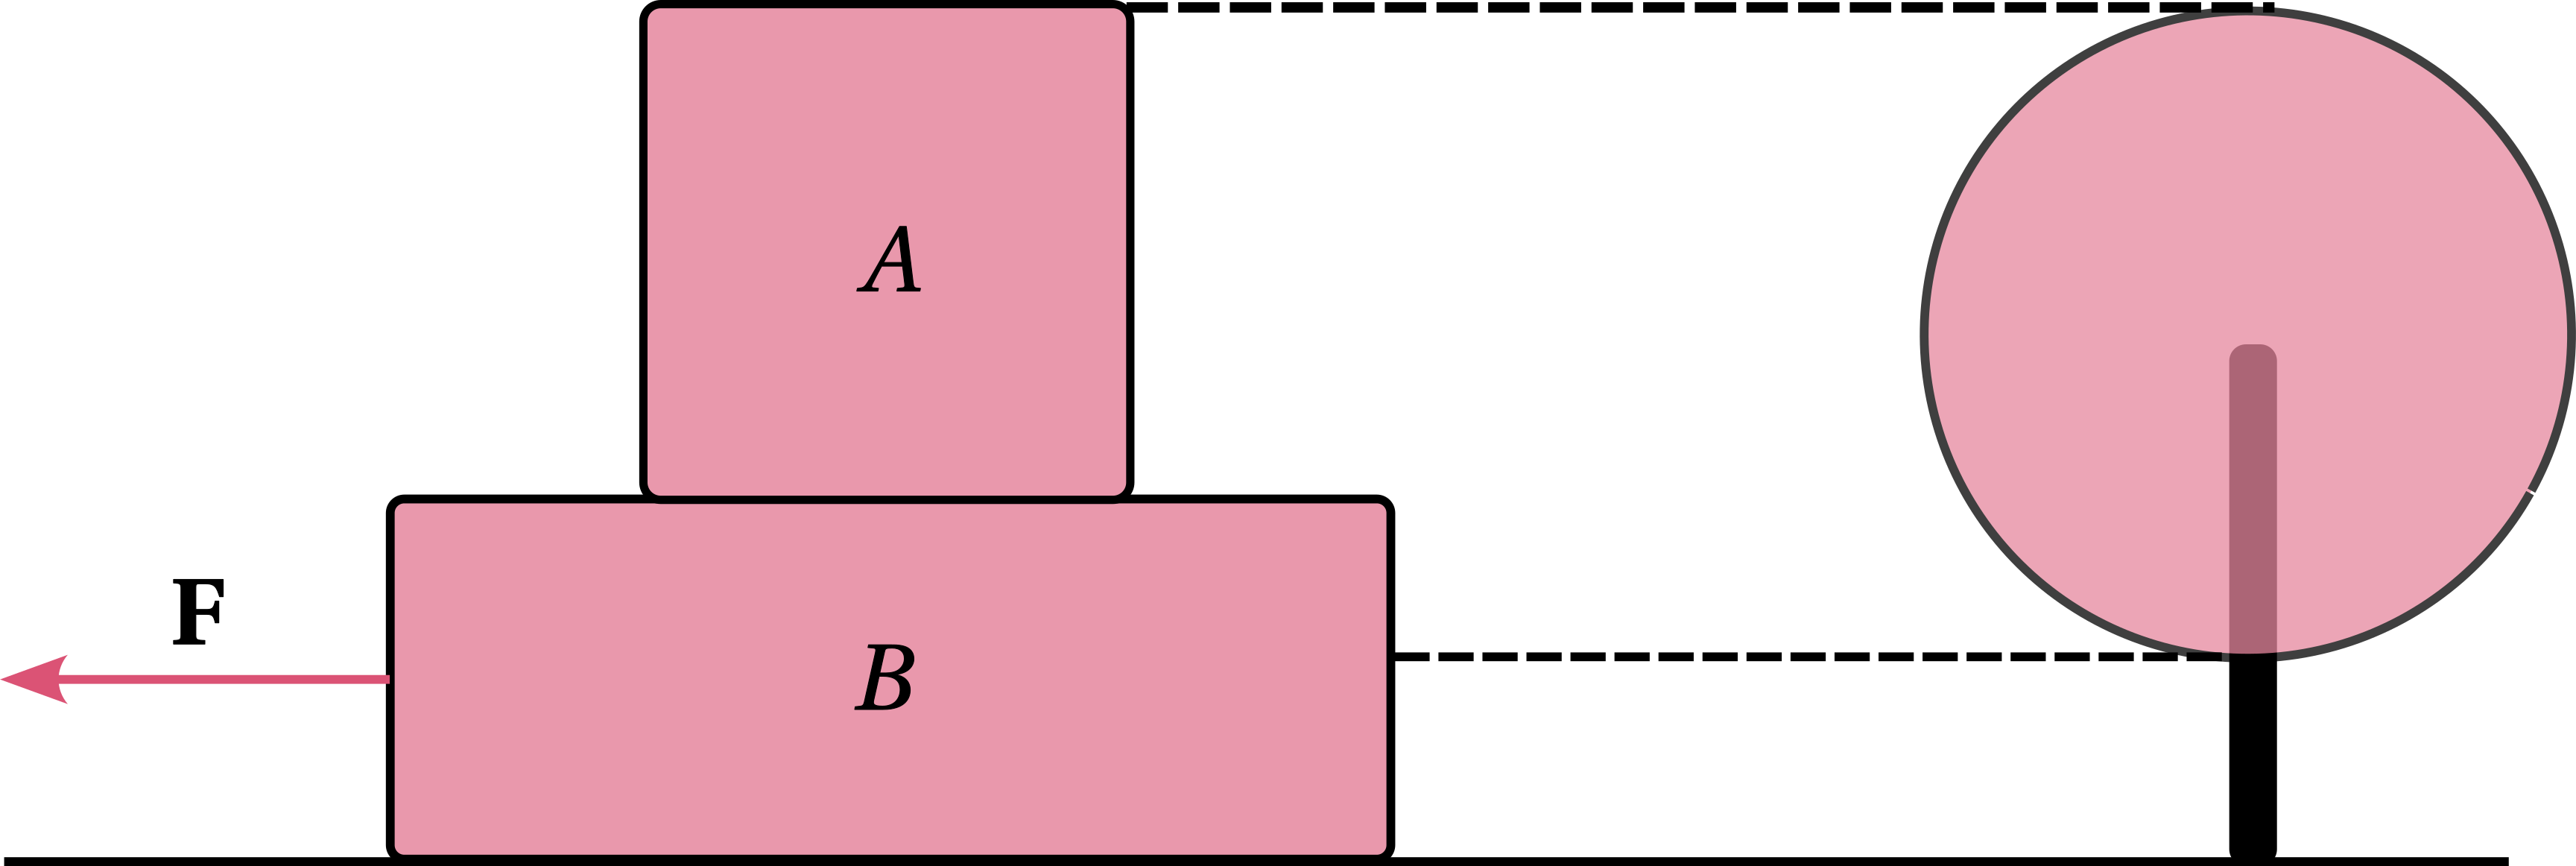
\includegraphics[width=0.58\textwidth]{assets/twoblocks.png}
  \caption{Two blocks and a pulley}
  \label{fig:twoblocks}
\end{wrapfigure}
We analyse the forces acting on block \(A\) first.

\section{Rod and trough}
\begin{problem}
  A uniform rod of weight \(\mv{W}\) and length \(L\) is supported at its ends
  by a frictionless trough, as shown in.
  Show that the centre of gravity of the rod is directly over point \(O\) when
  the rod is in equilibrium.
\end{problem}

We first define our variables. Let
\begin{itemize}
  \item the horizontal distance from the left end of the rod to point
    \(O\) be \(d_1\), and the horizontal distance from the right end
    of the rod to point \(O\) be \(d_2\);
  \item the normal contact force exerted by the trough on the left
    end of the rod be \(\mv{F}_1\), and
    that exerted by the trough on the right end of the rod be \(\mv{F}_2\);
  \item the angle the corner of the trough makes with respect to the
    left end be \(\alpha=\qty{30}{\degree}\),
    and that the trough makes with respect to the right end by
    \(\beta=\qty{60}{\degree}\).
\end{itemize}

For the rod to remain in equilibrium, \term{translational equilibrium}
and \term{rotational equilibrium}
must be attained. In translational equilibrium, the \it{vertical}
forces must sum to
zero, i.e. \(\sum\mv{F}_y = 0\).
We obtain the following, taking upwards as \(+y\):
\begin{equation}
  \sum\mv{F}_y = \mv{F}_1\cos\alpha + \mv{F}_2\cos\beta - \mv{W} = 0
  \label{eq:f1f2}
\end{equation}

In rotational equilibrium, the sum of moments about a fixed pivot
must equal \(0\).
We choose \(O\) as the pivot.
Assuming that the centre of gravity is a horizontal distance \(x\)
away from the pivot,
\begin{equation}
  \sum\tau =\mv{F}_1d_1\cos\alpha - \mv{F}_2d_2\cos\beta  + \mv{W}x = 0
  \label{eq:f1f2t}
\end{equation}

From \cref{eq:f1f2t}, we learn that
\begin{equation*}
  x = \f{\mv{F}_2d_2\cos\beta - \mv{F}_1d_1\cos\alpha}{\mv{W}}
\end{equation*}

From \cref{eq:f1f2}, we also learn that
\begin{equation*}
  \mv{F}_1 = \f{\mv{W} - \mv{F}_2\cos\beta}{\cos\alpha}
\end{equation*}
Substituting this into the above, we obtain
\begin{align*}
  x &= \f{\mv{F}_2d_2\cos\beta - \mv{F}_1d_1\cos\alpha}{\mv{W}} \\
  &= \f{1}{\mv{W}} \ab(\mv{F}_2d_2\cos\beta -
    \f{\mv{W}-\mv{F}_2\cos\beta}{\cancel{\cos\alpha}}\cdot
  d_1\cancel{\cos\alpha}) \\
  &= \f{1}{\mv{W}} \ab[\ab(d_1+d_2)\mv{F}_2\cos\beta - \mv{W}d_1]
\end{align*}

Notice anything? The expression in \it{square brackets} is the sum of moments
about a new pivot, the left end of the rod! Since the rod is in
rotational equilibrium,
this sum of moments should equal \(0\) as well, causing the rod to stay still.
We can conclude that
\begin{align*}
  x
  &= \f{1}{\mv{W}} \ab[\ab(d_1+d_2)\mv{F}_2\cos\beta - \mv{W}d_1] \\
  &= \f{1}{\mv{W}} \sum\tau \\
  &= \hil{0}
\end{align*}
Since the point at which the weight acts on the rod is a distance of \(x = 0\)
away from \(O\), \hil{the centre of gravity is \it{exactly} above \(O\)}.

\begin{problem}
  Determine the equilibrium value of the angle \(\theta\).
\end{problem}

\section{Wall push}
\begin{problem}
  In \cref{fig:wallpush}, a block of mass \(m = \qty{3.0}{\kg}\) is
  pushed up against a wall by a force
  \(\mv{P}\) that makes an angle \(\theta\) with respect to the horizontal.
  The coefficient of static friction between the block and the wall
  is \(\mu_s\).
  The frictional force acting on the block by the wall is \(\mv{f} =
  \mu_s\mv{R}\),
  where \(\mv{R}\) is the normal contact force acting on the block by the wall.

  Ensuring that the block stays at rest against the wall, what are the minimum
  and maximum values of \(\mv{P}\)?
\end{problem}
\begin{wrapfigure}{o}{0.5\textwidth}
  \centering
  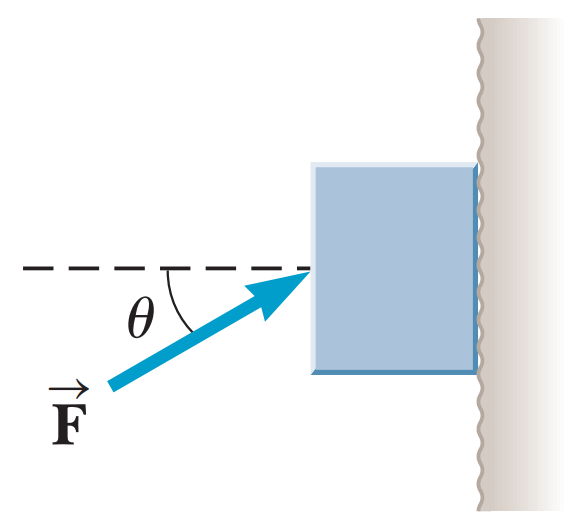
\includegraphics[width=0.48\textwidth]{assets/wallpush.png}
  \caption{Block pushed against wall}
  \label{fig:wallpush}
\end{wrapfigure}

We can first identify all the forces acting on the block and construct
a \term{free-body diagram}, in \cref{fig:wallpusha}.
\begin{wrapfigure}{i}{0.5\textwidth}
  \centering
  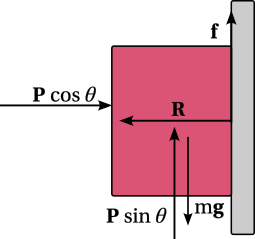
\includegraphics[width=0.48\textwidth]{assets/wallpush-annotated.png}
  \caption{Block pushed against wall (annotated)}
  \label{fig:wallpusha}
\end{wrapfigure}

Since the mass is in equilibrium, all horizontal and vertical forces
sum to \(0\), as in \cref{eq:blockhorz,eq:blockvert}.
\begin{align}
  \label{eq:blockhorz}
  \mv{P}\cos\theta&=-\mv{R} \\
  \mv{P}\sin\theta&=m\mv{g}-\mv{f}
  \label{eq:blockvert}
\end{align}
Combining \cref{eq:blockhorz,eq:blockvert}, we figure out that
\begin{align*}
  \mv{P}\sin\theta&=m\mv{g}-\mu_s\mv{R}\\
  &= m\mv{g}-\mv{P}\mu_s\cos\theta \\
\end{align*}
We get an expression for \(\mv{P}\), \cref{eq:blockp}.
\begin{equation}
  \mv{P} = \f{m\mv{g}}{\sin\theta + \mu_s\cos\theta}
  \label{eq:blockp}
\end{equation}
Since \(\ab|\mv{P}|\) is inversely proportional to
\(s\ab(\theta)=\sin\theta + \mu_s\cos\theta\),
the minimum value of \(s\ab(\theta)\) will produce a maximum
\(\mv{P}\), and vice versa.
We can differentiate to find the minimum and maximum values of \(s\ab(\theta)\):
\begin{align*}
  \odv{s\ab(\theta)}{\theta} &= \cos\theta-\mu_s\sin\theta\\
  &= \sqrt{1 + {\mu_s}^2}\cos\ab(\theta+\arctan\mu_s)
\end{align*}
At \(\odv{s\ab(\theta)}{\theta}=0\), \hil{\(\theta_1 =
\lf{\pi}{2}-\arctan{\mu_s}\)} and
\hil{\(\theta_2 = \lf{3\pi}{2}-\arctan{\mu_s}\)}.

For these two values of \(\theta\), we obtain
\begin{align*}
  \mv{P}_{\max} &= \f{m\mv{g}}{s\ab(\theta_1)} \\
  &= \f{m\mv{g}}{\sqrt{1+{\mu_s}^2}} \\
  \mv{P}_{\min} &= \f{m\mv{g}}{s\ab(\theta_2)} \\
  &= -\f{m\mv{g}}{\sqrt{1+{\mu_s}^2}}
\end{align*}
Surprisingly, the minimum and maximum values of \(\mv{P}\) are equal
in magnitude!
